\section{停止时刻与首次到达}
\label{sec:dtsp-stopping}
\label{sec:stoch-martingales-stopping-sequential-concentration}

很多观察不是运行固定步数后结束，而是“到某件事发生为止”：游走首次碰到边界，库存首次耗尽，算法的误差估计首次低于阈值。结束时刻因此是随机的。本节回答两个问题。第一，在随机时刻停止后，鞅的“期望不变”是否还成立，什么条件下成立；它给出到达概率和平均到达时间的计算方法。第二，Markov链在随机时刻停下后，未来是否仍像从当前状态重新开始；它是研究回返与长期平均的基础。

\subsection{停止规则与停止过程}
\label{sec:dtsp-stopping-rules}

\paragraph{只凭已有记录决定停止}
可执行的停止规则必须在每个时刻只根据已经看到的记录判断“现在停不停”。第~\ref{chap:stochastic-processes-and-sample-paths}章把这一要求写成：取值于$\mathbb N_0\cup\{\infty\}$的随机时刻$\tau$若对每个$n\geq0$都有$\{\tau\leq n\}\in\mathcal F_n$，就称为相对于$(\mathcal F_n)$的\term{停时}（stopping time），即停止时刻。离散时间中这等价于$\{\tau=n\}\in\mathcal F_n$对每个$n$成立，因为$\{\tau=n\}=\{\tau\leq n\}\setminus\{\tau\leq n-1\}$，而$\{\tau\leq n\}=\bigcup_{k\leq n}\{\tau=k\}$。

最常用的停时是首次到达。对可测集$A$，令$\tau_A=\inf\{n\geq0:X_n\in A\}$，则
\[
  \{\tau_A\leq n\}=\bigcup_{k=0}^n\{X_k\in A\}\in\mathcal F_n,
\]
到时刻$n$为止只需逐一检查已见的状态。常数时刻是停时；若$\sigma,\tau$是停时，则$\sigma\wedge\tau$、$\sigma\vee\tau$与$\tau+1$也是停时，例如$\{\sigma\wedge\tau\leq n\}=\{\sigma\leq n\}\cup\{\tau\leq n\}$。但$\tau-1$一般不是：在首次到达的前一刻宣布停止，需要预知下一步。同样，“在$0$到$N$之间路径取最大值的最后时刻”也不是停时，因为要确认某时刻之后再没有更高的值，必须看完整段路径。

\paragraph{停止过程}
在停时$\tau$处冻结一个过程，得到\term{停止过程}（stopped process）$M^{\tau}_n=M_{\tau\wedge n}$：$\tau$之前随原过程变化，之后保持在$M_\tau$不动。用鞅差写出来，
\begin{equation}
  M_{\tau\wedge n}=M_0+\sum_{k=1}^n\mathbb I\{\tau\geq k\}D_k.
  \label{eq:dtsp-stopped-process}
\end{equation}
冻结相当于从$\tau$之后把下注额设为零。由于$\{\tau\geq k\}=\{\tau\leq k-1\}^{\mathrm c}\in\mathcal F_{k-1}$，权重$H_k=\mathbb I\{\tau\geq k\}$可预测且有界，定理~\ref{thm:dtsp-martingale-transform}立即给出：鞅的停止过程仍是鞅，超鞅、次鞅的停止过程分别仍是超鞅、次鞅。冻结不破坏适应性，也不改变“每一步公平”这一性质。

\paragraph{停时处的信息}
停止以后，我们手里有哪些信息？直观上是“到$\tau$为止看到的一切”。把它写成$\sigma$代数：
\[
  \mathcal F_\tau=\{A\in\mathcal F:\ A\cap\{\tau\leq n\}\in\mathcal F_n\text{对每个}n\geq0\}.
\]
事件$A$属于$\mathcal F_\tau$，意思是在每个时刻$n$，只要已经停止，就能根据已有记录判断$A$是否发生。可以验证$\mathcal F_\tau$是$\sigma$代数；若$(X_n)$适应，则$X_\tau\mathbb I\{\tau<\infty\}$对$\mathcal F_\tau$可测，因为$\{X_\tau\in B\}\cap\{\tau=k\}=\{X_k\in B\}\cap\{\tau=k\}\in\mathcal F_k$。若$\sigma\leq\tau$，则$\mathcal F_\sigma\subseteq\mathcal F_\tau$：较早停止的人知道得较少。

\subsection{可选抽样与越界计算}
\label{sec:dtsp-optional-sampling}

\paragraph{有界停时}
既然停止过程仍是鞅，就有$\mathbb EM_{\tau\wedge n}=\mathbb EM_0$对每个固定的$n$成立。若$\tau$本身有上界$N$，取$n=N$便得到$\mathbb EM_\tau=\mathbb EM_0$。下面的定理把它推广到两个停时之间的条件期望。

\begin{theorem}[有界停时的可选抽样]
  \label{thm:dtsp-bounded-optional-sampling}
  设$(M_n)$是鞅，$\sigma\leq\tau\leq N$是两个停时，$N$为确定整数。则
  \[
    \mathbb E[M_\tau\mid\mathcal F_\sigma]=M_\sigma\qquad\text{几乎必然},
  \]
  特别地$\mathbb EM_\tau=\mathbb EM_0$。若$(M_n)$是次鞅（超鞅），等号换成$\geq$（$\leq$）。
\end{theorem}

\begin{proof}
$M_\sigma$对$\mathcal F_\sigma$可测，且$|M_\sigma|\leq\sum_{k\leq N}|M_k|$可积。只需对每个$A\in\mathcal F_\sigma$证明$\mathbb E[(M_\tau-M_\sigma)\mathbb I_A]=0$。由于$\sigma\leq\tau\leq N$，
\[
  (M_\tau-M_\sigma)\mathbb I_A=\sum_{k=1}^N\mathbb I_A\mathbb I\{\sigma<k\leq\tau\}D_k
  =\sum_{k=1}^N\mathbb I_{A\cap\{\sigma\leq k-1\}}\mathbb I\{\tau\geq k\}D_k.
\]
按$\mathcal F_\sigma$的定义，$A\cap\{\sigma\leq k-1\}\in\mathcal F_{k-1}$；又$\{\tau\geq k\}\in\mathcal F_{k-1}$。每一项的系数对$\mathcal F_{k-1}$可测，取期望后由$\mathbb E[D_k\mid\mathcal F_{k-1}]=0$为零。次鞅与超鞅情形中$\mathbb E[D_k\mid\mathcal F_{k-1}]$分别非负、非正，系数非负，得到相应不等式。
\end{proof}

证明清楚地标出了有界性的用途：它把随机长度的和改写成固定的有限和，从而可以逐项取期望。

\paragraph{从有界到无界：截断与极限交换}
实际的停时往往无界，例如“首次到达$1$”可能需要任意多步。自然的做法是先截断，再取极限：$\tau\wedge n$有界，所以$\mathbb EM_{\tau\wedge n}=\mathbb EM_0$；若$\tau<\infty$几乎必然，则$M_{\tau\wedge n}\to M_\tau$几乎必然。问题在于期望与极限能否交换。卷二已经建立了几乎处处收敛、依概率收敛与平均收敛的关系，控制收敛定理，一致可积条件下期望极限的交换，以及独立同分布序列的强大数律（可参考\BookChapterRef{chap:random-variable-convergence}{卷二“随机变量的收敛与积分极限”章}）。本章在这里和第~\ref{sec:dtsp-martingale-limits}、\ref{sec:dtsp-ergodic-averages}、\ref{sec:dtsp-iid-sampling}节调用这些结论。

\begin{theorem}[可选停止]
  \label{thm:dtsp-optional-stopping}
  设$(M_n)$是鞅，$\tau$是几乎必然有限的停时。若下列条件之一成立，则$M_\tau$可积且$\mathbb EM_\tau=\mathbb EM_0$：
  \begin{enumerate}
    \item 存在可积随机变量$Y$，使$|M_{\tau\wedge n}|\leq Y$对所有$n$成立；
    \item $\mathbb E\tau<\infty$，且存在常数$c$使$\mathbb E[|D_k|\mid\mathcal F_{k-1}]\leq c$对所有$k$成立；
    \item 停止过程$(M_{\tau\wedge n})_{n\geq0}$一致可积。
  \end{enumerate}
\end{theorem}

\begin{proof}
在每种条件下都从$\mathbb EM_{\tau\wedge n}=\mathbb EM_0$及$M_{\tau\wedge n}\to M_\tau$几乎必然出发。条件1下用控制收敛定理，条件3下用一致可积条件下的平均收敛，均得$\mathbb EM_{\tau\wedge n}\to\mathbb EM_\tau$。条件2化为条件1：取$Y=|M_0|+\sum_{k=1}^{\tau}|D_k|$，则$|M_{\tau\wedge n}|\leq Y$，且由非负项的换序与塔式性质，
\[
  \begin{aligned}
    \mathbb E\sum_{k=1}^{\tau}|D_k|&=\sum_{k\geq1}\mathbb E\bigl[\mathbb I\{\tau\geq k\}\,\mathbb E[|D_k|\mid\mathcal F_{k-1}]\bigr]\\
    &\leq c\sum_{k\geq1}\mathbb P(\tau\geq k)=c\,\mathbb E\tau<\infty.
  \end{aligned}
\]
这里$\{\tau\geq k\}\in\mathcal F_{k-1}$保证可以先对$D_k$取条件期望。
\end{proof}

三个条件从不同方向排除同一种危险：停止前的路径可能偏得极远，虽然概率很小，却把期望拉走了。只知道$\tau<\infty$几乎必然并不够。从$0$出发的公平游走，令$\tau=\inf\{n:S_n=1\}$。下面马上会证明$\tau<\infty$几乎必然，于是$S_\tau=1$，$\mathbb ES_\tau=1\neq0=\mathbb ES_0$。三个条件都不成立：$S_{\tau\wedge n}$向下无界，$\mathbb E\tau=\infty$，停止过程也不一致可积。

\paragraph{赌徒破产：到达概率与平均时间}
把游走限制在有界区间里，可选停止就成为计算工具。设$\pm1$游走向右概率为$p$、向左为$q=1-p$，从$k\in\{0,1,\ldots,N\}$出发，$\tau$为首次到达$0$或$N$的时刻。

第一步是确认$\mathbb E\tau<\infty$。从区间内任一点出发，连续向右$N$步必然离开区间，其概率为$p^N$。按长度$N$分块，每块独立地以至少$p^N$的概率结束，所以$\mathbb P(\tau>jN)\leq(1-p^N)^j$，$\mathbb E\tau\leq N/p^N<\infty$。

公平情形$p=1/2$。$S_n$是鞅，停止过程夹在$0$与$N$之间，条件1成立，于是$k=\mathbb ES_\tau=N\,\mathbb P_k(S_\tau=N)$，
\begin{equation}
  \mathbb P_k(\text{先到}N)=\frac kN.
  \label{eq:dtsp-ruin-fair}
\end{equation}
再用鞅$S_n^2-n$求平均时间。由有界停时的结论，$\mathbb E[S_{\tau\wedge n}^2]=k^2+\mathbb E[\tau\wedge n]$。令$n\to\infty$，左侧由有界收敛趋于$\mathbb ES_\tau^2=N^2\cdot k/N$，右侧由单调收敛趋于$k^2+\mathbb E\tau$，所以
\[
  \mathbb E_k\tau=k(N-k).
\]
从$N=10$的中点$k=5$出发平均需要$25$步，从$k=3$出发需要$21$步。

有漂移的情形$p\neq1/2$。$S_n$不再是鞅，但令$r=q/p$，乘积型过程$r^{S_n}$是鞅：$\mathbb E[r^{S_{n+1}}\mid\mathcal F_n]=r^{S_n}(pr+qr^{-1})=r^{S_n}(q+p)=r^{S_n}$。它在区间上有界，可选停止给出$r^k=\mathbb P_k(\text{先到}N)\,r^N+(1-\mathbb P_k(\text{先到}N))$，即
\begin{equation}
  \mathbb P_k(\text{先到}N)=\frac{1-r^k}{1-r^N}.
  \label{eq:dtsp-ruin-biased}
\end{equation}
取$N=10$、$k=3$、$p=0.47$，$r\approx1.128$，到达$10$的概率约为$0.187$，而公平时为$0.3$：每步$3\%$的劣势在十格的区间上被放大。图~\ref{fig:dtsp-gamblers-ruin}(b)把式~\eqref{eq:dtsp-ruin-fair}与\eqref{eq:dtsp-ruin-biased}同每个起点$4000$次模拟的频率放在一起。平均时间可用鞅$S_n-n(p-q)$同样求出：$\mathbb E_k\tau=(\mathbb E_kS_\tau-k)/(p-q)$。

\begin{figure}[htbp]
  \centering
  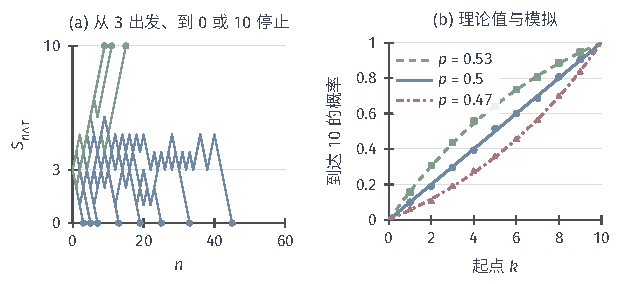
\includegraphics[width=105mm]{figures/03-optimization-evolution-and-signals/02-processes-and-trajectory-evolution/tikz/dtsp-gamblers-ruin/figure.pdf}
  \caption{赌徒破产问题。(a)公平游走从$3$出发、在首次到达$0$或$10$时停止的$14$条模拟路径（只画出$60$步内停止的路径），绿色为先到$10$；(b)先到$10$的概率随起点$k$的变化，曲线为式~\eqref{eq:dtsp-ruin-fair}与\eqref{eq:dtsp-ruin-biased}的精确值，标记为每个起点$4000$次模拟的频率。}
  \label{fig:dtsp-gamblers-ruin}
\end{figure}

\paragraph{首次到达的无界情形}
现在回到无界区间。公平游走从$0$出发，令$\sigma_m$为首次到达$1$或$-m$的时刻。由式~\eqref{eq:dtsp-ruin-fair}（把区间平移到$\{0,\ldots,m+1\}$，起点为$m$），先到$1$的概率是$m/(m+1)$，平均时间是$m\cdot1=m$。令$m\to\infty$：首次到达$1$的时刻$\tau$满足$\mathbb P(\tau<\infty)\geq m/(m+1)$对所有$m$成立，所以$\tau<\infty$几乎必然；又$\tau\geq\sigma_m$，故$\mathbb E\tau\geq m$对所有$m$成立，$\mathbb E\tau=\infty$。由对称性，从$1$出发首次回到$0$的时间期望也无穷，因此原点的平均返回时间$m_0=1+\mathbb E_1\tau_0=\infty$。这兑现了第~\ref{sec:dtsp-communication}节的说法：对称游走常返，但是零常返。

\paragraph{加倍下注：缺少条件的停止策略}
“公平游戏可以随意停止而仍然公平”并不是无条件的命题，加倍下注是最有名的反例。赌徒第一局押$1$，输了就把赌注加倍，直到第一次赢为止。若首胜出现在第$k$局，此前输掉$1+2+\cdots+2^{k-2}=2^{k-1}-1$，最后赢回$2^{k-1}$，净赢$1$。首胜几乎必然出现，所以$W_\tau=1$几乎必然，看起来是稳赚的系统。

矛盾出在哪里？每个截断时刻$n$，$W_{\tau\wedge n}$都是有界停时处的鞅值，期望为零。把它拆成已停与未停两部分：
\[
  \mathbb EW_{\tau\wedge n}=\underbrace{1\cdot\mathbb P(\tau\leq n)}_{1-2^{-n}}+\underbrace{(-(2^n-1))\cdot\mathbb P(\tau>n)}_{-(1-2^{-n})}=0.
\]
图~\ref{fig:dtsp-doubling-strategy}(b)画出这两项：未停部分的概率$2^{-n}$趋于零，它对期望的贡献却始终接近$-1$。极限中这份负质量“跑到了无穷远”，所以$\lim_n\mathbb EW_{\tau\wedge n}=0\neq1=\mathbb EW_\tau$。定理~\ref{thm:dtsp-optional-stopping}的三个条件都失败：亏损无下界，$\mathbb E\sum_{k\leq\tau}|D_k|=\sum_k2^{k-1}\cdot2^{-(k-1)}=\infty$，停止过程不一致可积。若赌徒有信用上限，最多连输$m$局，那么停止时刻有界为$m$，期望收益严格为零：以概率$1-2^{-m}$赢$1$，以概率$2^{-m}$输$2^m-1$。

\begin{figure}[htbp]
  \centering
  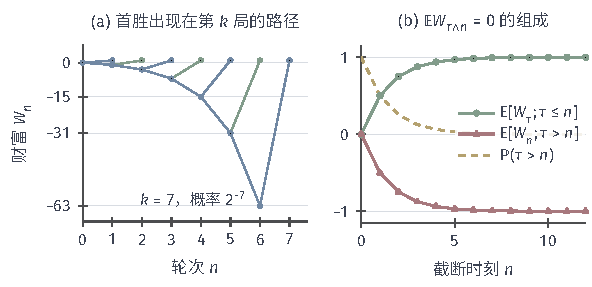
\includegraphics[width=100mm]{figures/03-optimization-evolution-and-signals/02-processes-and-trajectory-evolution/tikz/dtsp-doubling-strategy/figure.pdf}
  \caption{加倍下注（精确计算）。(a)首胜出现在第$k=1,\ldots,7$局时的财富路径，每条路径的概率为$2^{-k}$，终点都是$+1$；(b)截断期望$\mathbb EW_{\tau\wedge n}=0$的两个组成部分：已停部分$\mathbb E[W_\tau;\tau\leq n]=1-2^{-n}$与未停部分$\mathbb E[W_n;\tau>n]=-(1-2^{-n})$，以及未停概率$2^{-n}$。}
  \label{fig:dtsp-doubling-strategy}
\end{figure}

\subsection{停止后的Markov链}
\label{sec:dtsp-strong-markov}

\paragraph{强Markov性质}
可选抽样处理的是期望；现在研究停止后整个未来的条件分布。Markov性质说，在固定时刻$n$给定现在，未来像从$X_n$重新出发的链。若把$n$换成停时$\tau$，结论是否仍成立？对离散时间链，答案是肯定的，而且证明只需按$\tau$的取值拆开。记$\mathbb E_x$为从$x$出发、以$P$为转移核的链的期望，并先把定理~\ref{thm:dtsp-chapman-kolmogorov}推广到路径函数：对有界可测$g$，
\begin{equation}
  \mathbb E[g(X_n,X_{n+1},\ldots,X_{n+m})\mid\mathcal F_n]=\mathbb E_{X_n}[g(X_0,\ldots,X_m)]\qquad\text{几乎必然}.
  \label{eq:dtsp-markov-path}
\end{equation}
对乘积形式$g=\prod_jg_j(x_j)$，它由对$m$归纳、每次用一步转移核得到；一般的有界可测$g$再由单调类论证推出。

\begin{theorem}[离散时间的强Markov性质]
  \label{thm:dtsp-strong-markov}
  设$(X_n)$是以$P$为转移核的时间齐次Markov链，$\tau$是停时。则对每个$A\in\mathcal F_\tau$、每个$m\geq0$和每个有界可测$g$，
  \[
    \mathbb E\bigl[g(X_\tau,\ldots,X_{\tau+m})\,\mathbb I_A\,\mathbb I\{\tau<\infty\}\bigr]
    =\mathbb E\bigl[\mathbb E_{X_\tau}[g(X_0,\ldots,X_m)]\,\mathbb I_A\,\mathbb I\{\tau<\infty\}\bigr].
  \]
  也就是说，在$\{\tau<\infty\}$上给定$\mathcal F_\tau$，停止后的过程$(X_{\tau+n})_{n\geq0}$是从$X_\tau$出发、以$P$为转移核的Markov链。
\end{theorem}

\begin{proof}
把左侧按$\{\tau=n\}$拆成可数和。由$\mathcal F_\tau$的定义，$A\cap\{\tau=n\}\in\mathcal F_n$；在这个事件上$X_\tau=X_n$。对第$n$项使用式~\eqref{eq:dtsp-markov-path}，
\[
  \mathbb E\bigl[g(X_n,\ldots,X_{n+m})\mathbb I_{A\cap\{\tau=n\}}\bigr]
  =\mathbb E\bigl[\mathbb E_{X_n}[g(X_0,\ldots,X_m)]\,\mathbb I_{A\cap\{\tau=n\}}\bigr].
\]
再对$n$求和；$g$有界保证求和与期望可以交换。
\end{proof}

证明的关键是时间可数，可以把停时的每个取值单独处理。连续时间中停时可以取不可数多个值，这一拆分不再可用，强Markov性质还需要路径正则性等额外条件，第~\ref{chap:continuous-time-stochastic-processes}章将讨论。

\paragraph{回返与再生分段}
强Markov性质首先兑现了式~\eqref{eq:dtsp-visit-geometric}。令$T^{(k)}$为第$k$次回到$i$的时刻，它是停时，且$X_{T^{(k)}}=i$。在$\{T^{(k)}<\infty\}$上，链从$i$重新开始，再回来一次的条件概率仍是$f_i$，因此$\mathbb P_i(T^{(k+1)}<\infty)=f_i\,\mathbb P_i(T^{(k)}<\infty)=f_i^{k+1}$，这正是$\mathbb P_i(N_i>k+1)$。

更进一步，把一条常返路径在每次访问$i$处切开，得到一段段\term{游程}（excursion）：从一次访问$i$起、到下一次回到$i$之前为止。强Markov性质说明，每段游程给定此前全部历史的条件分布都等于从$i$出发的第一段游程的分布；因此各段游程独立同分布。路径被切成了一串独立同分布的“再生”片段，关于长时间平均的问题就可以借助独立同分布序列的强大数律处理，这正是第~\ref{sec:dtsp-ergodic-averages}节的证明思路。

两类停止结论回答不同的问题，使用时不能混淆。可选抽样给出期望等式，例如到达概率与平均时间，它需要可积性或有界性条件，不需要Markov性；强Markov性质给出停止后未来的完整条件分布，它需要Markov结构，但不涉及任何期望的有限性。
